\chapter{Konzept und Implementierung}\label{chap:concept}

\section{Konzept}\label{sec:concept}

Das Programmablauf wird in einzelne Schritte unterteilt, auf die in den nächsten Kapiteln näher eingegangen werden.
\\\\
\begin{figure}[ht]
  \centering
  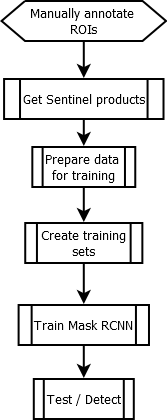
\includegraphics[width=.2\textwidth]{pics/overview.PNG}
  \caption{Gesamtablauf der Anwendung}
  \label{fig:overview}
\end{figure}
Zuerst müssen die Daten für das Training bzw. für die Erkennung manuell annotiert werden. Diese Metadaten werden dann genutzt, um automatisch Sentinelprodukte\footnote{Aufnahmenpakete der Sentinel-Plattformen werden als Produkte bezeichnet.} mittels einer API, die von der Copernicus zur Verfügung gestellt wird, herunterzuladen. Aus den Produkten werden die relevanten Bänder extrahiert und unter anderem die jeweiligen NDVI-Werte berechnet. Nachdem die Produkte für das Training vorbereitet wurden, werden die Daten in ein Trainings- und in ein Validierungsdatensatz aufgeteilt. Der folgende Trainingsprozess basiert auf diesen Datensätzen. Sobald das Training abgeschlossen ist, kann die Performanz des Modells getestet werden. 

\section{Annotation}\label{sec:annotation}

Zu Beginn werden die Regionen, die entweder für das Training benutzt oder überprüft werden, manuell erfasst. Vorrausgesetzte Informationen sind
\begin{itemize}
	\item Geografische Koordinaten,
	\item Zeitraum des Befalls und
	\item Bezeichnung der Infektion.
\end{itemize}
Als Format dieser Informationen dient \textit{GeoJSON}\footnote{GeoJSON ist eine Erweiterung des JSON-Format und beschreibt geografische Daten und Geometrien. GeoJSON wird durch den RFC7946-Standard definiert.}. GeoJSON enthält nicht nur geografische Daten, sondern ist auch um benutzerdefinierte Eigenschaften (\texttt{properties}) erweiterbar.

\begin{lstlisting}[language=json,caption={Annotation},captionpos=b]
{
  "type": "Feature",
  "properties": {
    "disease": 1,
    "from": "2018-07-12T13:00:00Z-7DAYS",
    "to": "2018-07-12T13:00:00Z+7DAYS"
  },
  "geometry": {
    "type": "Polygon",
    "coordinates": [[[11.171988617177981,44.574291380353003],
       [11.1726616444942,44.574017992242283],
       [11.17338129910439,44.575068359984279],
       [11.17273129334275,44.575299863118993],
       [11.171988617177981,44.574291380353003]]]
  }
}
\end{lstlisting}
\noindent
\texttt{properties.disease} enthält die eindeutige, nummerische Repräsentation der Klasse bzw. Krankheit, die in dieser Region enthalten ist. Die Zuordnung der nummerischen Werte und des textuellen Bezeichners werden in einer separaten JSON als Schlüssel-Wert-Paare konfiguiert, wobei der Schlüssel nummerisch und der Wert textuell ist. Hier ist, darauf zu achten, dass der Schlüssel $\ge1$ ist, da $0$ der implizite Schlüssel der Mask R-CNN-Implementierung für den Hintergrund ist. Diese Eigenschaft ist nur für das Training von Relevanz.
\\\\
\texttt{properties.from} und \texttt{properties.to} sind jeweils Start- und Endzeitpunkt, in dem nach verfügbaren Sentinelprodukten gesucht werden soll. Das Format der jeweiligen Eigenschaften kann eine der folgenden Formen haben\footnote{Die Formate basieren auf der \texttt{sentinelsat}-Version 0.12.2.}:
\begin{itemize}
	\item \texttt{yyyyMMdd}
	\item \texttt{yyyy-MM-ddThh:mm:ss.SSSZ} (ISO-8601)
	\item \texttt{yyyy-MM-ddThh:mm:ssZ}
	\item \texttt{NOW}
	\item \texttt{NOW-<n>DAY(S)} (oder \texttt{HOUR(S)}, \texttt{MONTH(S)}, usw.)
	\item \texttt{NOW+<n>DAY(S)}
	\item \texttt{yyyy-MM-ddThh:mm:ssZ-<n>DAY(S)}
	\item \texttt{NOW/DAY} (oder \texttt{HOUR}, \texttt{MONTH} usw.) - Der Wert wird auf den jeweiligen Typ (z.B. auf den Tag) gerundet.
\end{itemize}

\section{Suche der Sentinelprodukte}

\begin{figure}[ht]
  \centering
  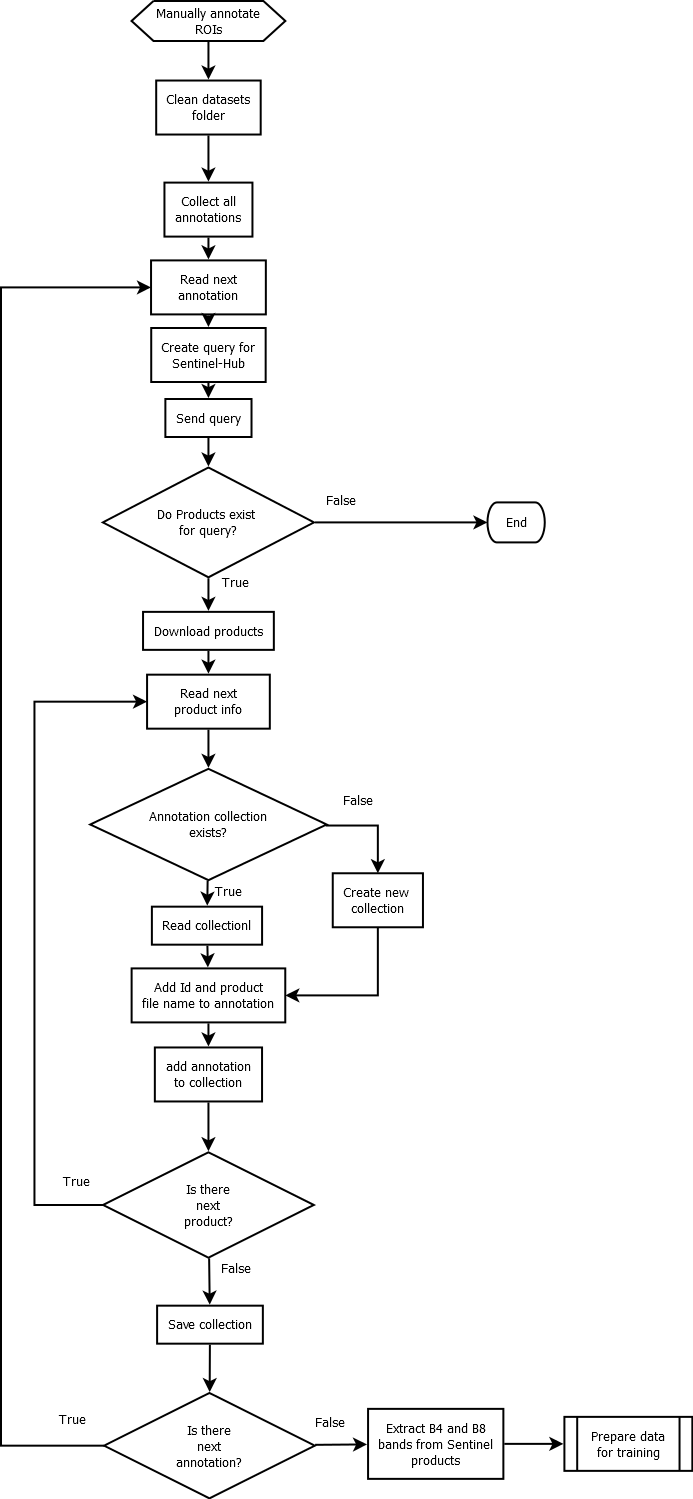
\includegraphics[width=.65\textwidth]{pics/get-products.png}
  \caption{Ablaufdiagramm der Beschaffung der Sentinelprodukte}
  \label{fig:get-products}
\end{figure}

Der \textit{Copernicus Open Access Hub}\footnote{\url{https://scihub.copernicus.eu/}} ermöglicht freien und offenen Zugriff auf Sentinel-Produkte. Die Daten sind sowohl über eine grafische Oberfläche als auch über eine REST-API verfübar. Vorrausgesetzung für beide Optionen ist ein Account, der über die grafische Oberfläche erstellt werden kann.
\\\\
Die Nutzung der Schnittstelle erfolgt über die Python-Bibliothek \texttt{sentinelsat}\footnote{https://sentinelsat.readthedocs.io/en/stable}. Bei einer Anfrage müssen die GeoJSON-Dateien in WKT\footnote{WKT (Well-known text) ist eine Markup-Sprache zur Repräsentation von geometrischen Objekten auf Karten und räumlichen Referenzsystemen.} umgewandelt werden, was von der Bibliothek übernommen werden kann. 

\todo{Liste}